%		tutorial
%		========
%
%	This chapter gives an overview of the features 
%	and a howto to obtain most kinds of plots.

\chapter{Drawing plots with \SciDaVis}

%		2D X-Y plots
%		============

\section{2D X-Y plots}\label{sec-2d-plots}

\index{Plot}
A 2D plot is based on curves which are defined by $Y$ values as
functions of $X$ values. There are different ways to obtain a 2D plot
depending on the way the $(X,Y)$ values are defined:


\begin{enumerate}
  \item You can have your (X,Y) values in a
  \htmlref{table}{sec-intro-table}. You need to select at least one
  column as X values and one column as Y values. This is specified
  with the \htmlref{Set Column As command}{set-column-as-lnk}. Then you can
  select the columns and use one command of the \htmlref{Plot
  menu}{plot-menu-lnk} to plot the data.
  \item If you want to plot a function, you don't need a table. You
  can use directly the \htmlref{New Function Plot
  command}{new-function-plot-lnk}. This will open the corresponding
  dialog box and you will be able to define the mathematical
  expression of your function. In this case, plot can be obtained from
  functions in cartesian coordinates $Y(X)$, but also in parametered
  coordinates $(X(t),Y(t))$, or in angular coordinates $r(\theta)$. 
  \item The combined way is to define a
  \htmlref{table}{sec-intro-table}, and then to fill in the table with
  the results of functions. This can be done with the \htmlref{Assign
  Formula command}{assign-formula-lnk}. Then you can select the
  columns and use one command of the \htmlref{Plot
  menu}{plot-menu-lnk} to plot the data.
  \end{enumerate}  

\SciDaVis{} will create a new graph window, and the plot will be
inserted in a new layer.

Once the plot is created, you can customize all the graphic items of the plot with the commands of the \htmlref{Format Menu}{sec-format-menu}. You can add new items (text labels, lines or arrows, new legend, images) on the plot with the commands of the \htmlref{Graph Menu}{sec-graph-menu}.

%============================================================================
%
%		how to obtain a 2D plot from a table
%

\subsection{2D plot from data.}\label{sec-2d-plot-from-data}
\index{Plot!Create from data}
The data must be stored in a \htmlref{table}{sec-intro-table}. There
are several possibilities to insert your $(X,Y)$ values in the table:
you can write them directly from the keyboard, or read them from a
file. Here we will use the first solution, refer to the
\htmlref{Import ASCII command}{import-ascii-lnk} to use the second one.

The first step is to create an empty project with the \htmlref{New
Project command}{new-project-lnk} from the \htmlref{File
menu}{file-menu-lnk}, you can also use the key \htmlref{New Project
key}{new-project-key} or the \icon{new.png} icon from the \htmlref{File
toolbar}{file-toolbar-lnk}. Then create a new table with the
\htmlref{New Table command}{new-table-lnk} from the \htmlref{File
menu}{file-menu-lnk} or with the \htmlref{New Table
key}{new-table-key} or with the \icon{table.png} icon from the \htmlref{File toolbar}{file-toolbar-lnk}.

At its creation, the table has two column (one for $X$ and one for
$Y$) and 32 rows. You can add rows and columns by selecting a row or a
column and using the right button of the mouse, you can also modify
the number of rows and columns with the \htmlref{Table Dimensions
command}{table-dimensions-lnk} from the \htmlref{Table menu}{table-menu-lnk}. Then, enter your values, and you obtain the table shown in figure \ref{fig-simple-2dplot-1}.

\begin{figure}
  \resizebox{\textwidth}{!}{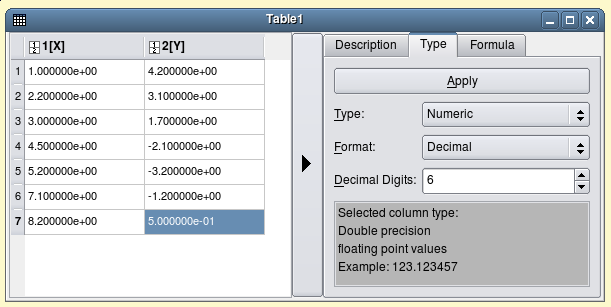
\includegraphics{tutorial/simple-2dplot-1.png}}
  \caption{A simple 2D plot: the table.}
  \label{fig-simple-2dplot-1}
\end{figure}

Then, you have to select the two columns, and build your plot (here a
simple 2D scatter) with the \htmlref{Scatter command}{scatter-lnk}
from the context menu, or by clicking on the corresponding
\icon{pPlot.png} icon from the \htmlref{Plot
toolbar}{plot-toolbar-lnk} or with the \htmlref{Scatter
command}{scatter-lnk} from the \htmlref{Plot menu}{plot-menu-lnk}. A
plot is created which uses the default options for all elements. You
can customize these default options with the \htmlref{2D plot
preferences dialog}{sec-preferences-2d-plot}. With the default
options, you obtain the plot shown in figure
\ref{fig-simple-2dplot-2}.

\begin{figure}
  \resizebox{\textwidth}{!}{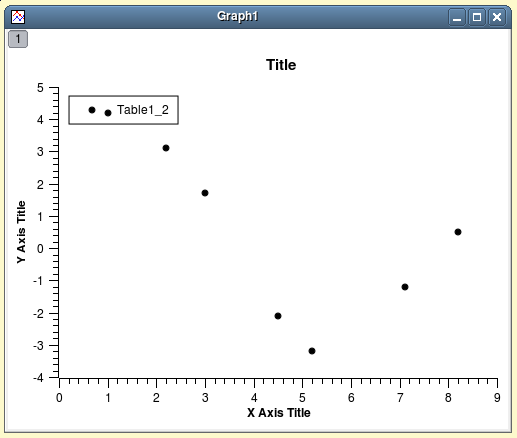
\includegraphics{tutorial/simple-2dplot-2.png}}
  \caption{A simple 2D plot: the default plot.}
  \label{fig-simple-2dplot-2}
\end{figure}

You can now customize your plot with the commands of the
\htmlref{Format menu}{format-menu-lnk}. By double clicking on the data
points, you open the \htmlref{Format plot}{format-plot-lnk} dialog
which is used to modify the symbols. Then a double-click on the axes
opens the \htmlref{Format Axes}{format-axes-lnk} dialog, and you can
change the scales, the fonts for the axes labels, etc. You can also
add grid lines on $X$ or $Y$ axes (\htmlref{Format Grid}{format-grid-lnk}), etc. Finally, a double click on each text item ($X$ title, $Y$ title, plot title) allows to change the text and the presentation of these elements. See the \htmlref{customize section}{sec-customize-2d-plot} for more details. An example of the final plot is shown in figure \ref{fig-simple-2dplot-3}.
%
%<figure id="fig-simple-2dplot-3">
%  <title>A simple 2D plot: the plot finished.</title>
%  <mediaobject> 
%    <imageobject>
%      <imagedata  format="PNG" fileref="tutorial/simple-2dplot-3.png"/>
%    </imageobject>
%  </mediaobject>
%</figure>
\begin{figure}
  \resizebox{\textwidth}{!}{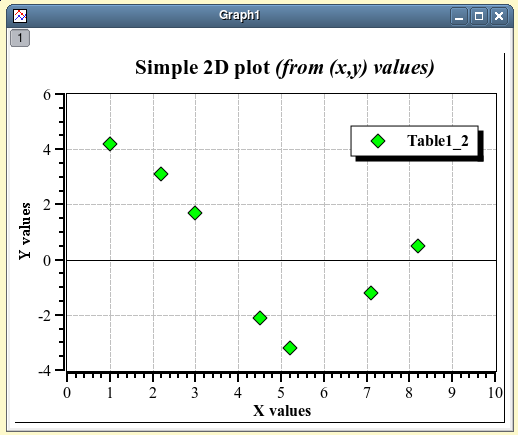
\includegraphics{tutorial/simple-2dplot-3.png}}
  \caption{A simple 2D plot: the plot finished.}
  \label{fig-simple-2dplot-3}
\end{figure}

Finally, you have to save your project in a '.sciprj' file with the
\htmlref{Save Project}{save-project-lnk} from the \htmlref{File
  menu}{file-menu-lnk} or with \html{CTRL+S}{save-project-key} or with
the \icon{filesave.png} icon from the \htmlref{File
  toolbar}. Depending on your application, you can export your plot to
a standard image file with the command  \htmlref{Export
  Graph$\rightarrow$Current command}{export-graph-current-lnk} from
the \htmlref{File menu}{file-menu-lnk} (or with the \htmlref{CTRL+G}{export-graph-current-key} keycode).

\index{Plot!secondary axis}

There are several types of plots which can be built from a table. They
are presented in the \htmlref{Plot menu}{plot-menu-lnk}. One important
feature is that it is possible to use up to four axis for the
data. For example, create a new table, modify its dimension to 4
columns and 7 rows. Then select the third column and set it as $X$
with the \htmlref{Set Column as command}{set-column-as-lnk} from the
\htmlref{Table menu}{table-menu-lnk}; you can then enter the values of two series $(X1,Y1)$ and $(X2,Y2)$ as shown in the figure \ref{fig-two-axes-plot}.
%
%<figure id="fig-two-axes-plot">
%  <title>A table with two series of values (X1,Y1) and (X2,Y2).</title>
%  <mediaobject> 
%    <imageobject>
%      <imagedata  format="PNG" fileref="tutorial/2axes-2dplot-1.png"/>
%    </imageobject>
%  </mediaobject>
%</figure>
\begin{figure}
  \resizebox{\textwidth}{!}{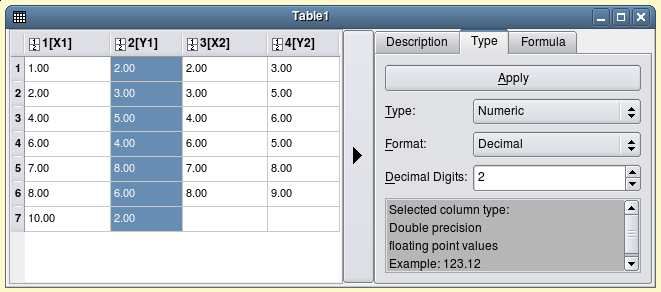
\includegraphics{tutorial/2axes-2dplot-1.png}}
  \caption{A table with two series of values $(X1,Y1)$ and $(X2,Y2)$.}
  \label{fig-two-axes-plot}
\end{figure}

To build the plot, select the two $Y$ columns (select $Y1$, and then
select $Y2$ with CTRL key), use the \htmlref{Plot
  menu}{plot-menu-lnk}. You obtain a simple plot with two axes, then
use the \htmlref{Format Plot}{format-plot-lnk}. In the left window,
select the data serie for which you want to change the axes, click on
the {\em axis} tag and define the axes you want to use. After this,
the plot is modified but the new axes are not shown. Use the
\htmlref{Format Axes command}{format-axes-lnk}, select the new axes
and click on the {\em show} checkbox. You can then customize your plot in order to obtain the result presented in figure \ref{fig-two-axes-plot-1}.


%
%<figure id="fig-two-axes-plot-1">
%  <title>A 2D plot with two Y and two X axis.</title>
%  <mediaobject> 
%    <imageobject>
%      <imagedata  format="PNG" fileref="tutorial/2axes-2dplot-2.png"/>
%    </imageobject>
%  </mediaobject>
%</figure>
\begin{figure}
  \resizebox{\textwidth}{!}{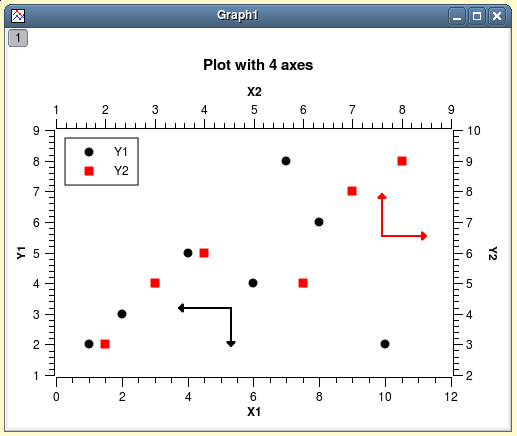
\includegraphics{tutorial/2axes-2dplot-2.png}}
  \caption{A 2D plot with two Y and two X axis.}
  \label{fig-two-axes-plot-1}
\end{figure}

In addition to the customization which has been already described,
four arrows were added with the \htmlref{Draw arrow}{draw-arrow-lnk}.


%		how to obtain a 2D plot from a function
\subsection{2D plot from function.}
\label{sec-2d-plot-from-function}
\index{Plot!Create from function}

There are two ways to obtain such a plot: you can plot directly a
function or fill a table with the values calculated from this function
before doing a plot in the classical way.

\subsubsection{Direct plot of a function.}

If you just want to plot a function, you can use the
\htmlref{New Function Plot}{new-function-plot-lnk} from the
\htmlref{File Menu}{file-menu-lnk} or with the
\htmlref{New Function Plot Key}{new-function-plot-key} or with the
\htmlref{New Function Plot}{new-function-plot-icon} icon from
the \htmlref{File toolbar}{file-toolbar-lnk}.

You can then enter the expression of your mathematical function, the $X$
range used for the plot, and the number of points used in this $X$
range. See the \htmlref{Add Function}{add-function-lnk} for details.

\begin{figure}
  \resizebox{\textwidth}{!}{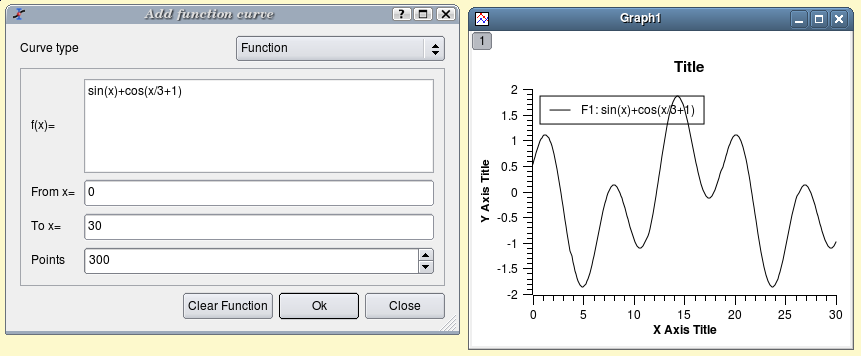
\includegraphics{tutorial/direct-function-plot.png}}
  \caption{Direct plot of a function.}
  \label{fig-direct-function-plot-1}
\end{figure}
%<figure id="fig-direct-function-plot-1">
%  <title>Direct plot of a function.</title>
%  <mediaobject> 
%    <imageobject>
%      <imagedata  format="PNG" fileref="tutorial/direct-function-plot.png"/>
%    </imageobject>
%  </mediaobject>
%</figure>
%


The generic plot which is created by this command can then be
customized as explained in the previous section. Beside classical
$Y=f(X)$ functions, parametric functions and polar functions can be
defined. In parametric coordinates, $X$ and $Y$ are defined as
functions of an independant parameter $m$. You can define these
functions, the range for $m$ and the number of points computed in this
range.

%
%<figure id="fig-direct-function-plot-2">
%  <title>Direct plot of a parametric function.</title>
%  <mediaobject> 
%    <imageobject>
%      <imagedata  format="PNG" fileref="tutorial/direct-function-plot-parametric.png"/>
%    </imageobject>
%  </mediaobject>
%</figure>
%
%<para>Polar coordinate are defined as a radius <emphasis>R</emphasis> and an angle <emphasis>theta</emphasis> (in radian). The coordinates are then obtained by <emphasis>X=R.cos(theta)</emphasis> and <emphasis>Y=R.sin(theta)</emphasis>. You can use a parametric definition: <emphasis>R=f(t)</emphasis> and  <emphasis>theta=f(t)</emphasis>, the range for <emphasis>t</emphasis> and the number of points computed in this range.</para>
%
%<figure id="fig-direct-function-plot-3">
%  <title>Direct plot of a function in polar coordinates.</title>
%  <mediaobject> 
%    <imageobject>
%      <imagedata  format="PNG" fileref="tutorial/direct-function-plot-polar.png"/>
%    </imageobject>
%  </mediaobject>
%</figure>
%
%</sect3>
%<!--
%**********************************************************************
%
%		filling of a table with a function
%
%**********************************************************************
%-->
%<sect3 id="sec-table-function-plot">
%<title>Filling of a table with the values of a function.</title>
%
%<indexterm>
%  <primary>Columns</primary><secondary>Assign formula</secondary>
%</indexterm>
%<para>If you just want to work not only with the plot but also with the data, you can create a new table as explained in the <link linkend="sec-2d-plot-from-data">previous section</link>. Then you can fill this table with the values of a function with the &assign-formula-lnk;. The main advantage of this method is that you can do further analysis of the calculated data as the are kept in a table.</para>
%
%<para>To obtain the same plot as in the previous example, you need to create a new table (key &new-table-key;) and use the &table-dimensions-lnk; to define 300 rows, then select the first column and use the command &assign-formula-lnk; from the context menu, or from the &table-menu-lnk;. The row number symbol is <emphasis>i</emphasis>, so you can enter the function expression <emphasis>i/10</emphasis> (figure <xref xrefstyle="select: labelnumber" linkend="fig-table-function-plot-1"/>).</para>
%
%<figure id="fig-table-function-plot-1">
%  <title>Function plot: filling of the X column.</title>
%  <mediaobject> 
%    <imageobject>
%      <imagedata  format="PNG" fileref="tutorial/table-function-plot1.png"/>
%    </imageobject>
%  </mediaobject>
%</figure>
%
%<para>The second step is to select the second column and use the same command. The expression is a function of the X values, that is the first column named <emphasis>col(1)</emphasis> (figure <xref xrefstyle="select: labelnumber" linkend="fig-table-function-plot-2"/>).</para>
%
%<figure id="fig-table-function-plot-2">
%  <title>Function plot: filling of the Y column.</title>
%  <mediaobject> 
%    <imageobject>
%      <imagedata  format="PNG" fileref="tutorial/table-function-plot2.png"/>
%    </imageobject>
%  </mediaobject>
%</figure>
%
%<para>Once the table is ready, you just have to build the plot as explained in the previous section.</para>
%
%</sect3>
%
%</sect2>
%
%<!--
%*******************************************************************
%
%		Other 2D plots
%		**************
%
%*******************************************************************
%-->
%<sect2 id="sec-other-2d-xy-plot">
%<title>The different types of 2D X-Y plots</title>
%
%<para>Beside the conventional X-Y plots with lines and points, other kinds of plots are available in &appname;. Although the presentation of the data can be very different, they are all based on the use of one column for X values and one column for Y values. Follow the links to the corresponding commands to see a description of these plots.</para>
%
%<para>The first set is available in the subset <emphasis>Special Lines/Symbol</emphasis> of the &plot-menu-lnk;:</para>
%
%<itemizedlist>
%  <listitem>
%    <para>Drop lines plot (&vertical-drop-lines-lnk;)</para>
%  </listitem>
%  <listitem>
%    <para>Scatter plot with a smoothed line connection between the points (&spline-lnk;)</para>
%  </listitem>
%  <listitem>
%    <para>Vertical steps plot (&vertical-steps-lnk;)</para>
%  </listitem>
%  <listitem>
%    <para>Horizontal steps plot (&horizontal-steps-lnk;)</para>
%  </listitem>
%</itemizedlist>
%<para>The other ones are more special plots which can be accessed directly in the &plot-menu-lnk;:</para>
%<itemizedlist>
%  <listitem>
%    <para>Vertical bars plot (&columns-lnk;)</para>
%  </listitem>
%  <listitem>
%    <para>Horizontal bars plot (&rows-lnk;)</para>
%  </listitem>
%  <listitem>
%    <para>Area plot (&area-lnk;)</para>
%  </listitem>
%</itemizedlist>
%
%</sect2>
%
%<!--
%*******************************************************************
%
%		customization of 2D plots
%		*************************
%
%*******************************************************************
%-->
%<sect2 id="sec-customize-2d-plot">
%<title>Customization of a 2D plot</title>
%
%<para>There are many way to improve and modify the plots:</para>
%<itemizedlist>
%  <listitem>
%    <para>The first part of the commands are used to modify the main elements of the plot, that is axis, labels, etc. They can be accessed through the &format-menu-lnk;.</para>
%  </listitem>
%  <listitem>
%    <para>The second part of commands can be used to insert additional objects likes arrows, images, text labels, etc. They can be accessed in the &graph-menu-lnk;.</para>
%  </listitem>
%</itemizedlist>
%<para>This section will show an overview of the first set of commands. See the &graph-menu-lnk; section for the other commands. There are three main windows which allows to modify the plot:</para>
%<itemizedlist>
%  <listitem>
%    <para>The &format-plot-lnk;, it is entitled "Plot details" and is used to customize the global properties of the plot (background color, etc) and the data series (points shape, line width, etc).</para>
%  </listitem>
%  <listitem>
%    <para>The second one is entitled "General plot options" and contain the commands to format axes (scales, labels, grids, etc), it can be accessed through the &format-scales-lnk;, &format-axes-lnk; and &format-grid-lnk;.</para>
%  </listitem>
%  <listitem>
%    <para>The last one is the &format-title-lnk; which is used to control the properties of the title of the plot.</para>
%  </listitem>
%</itemizedlist>
%<para>All these commands are accessed through the &format-menu-lnk;.</para>
%
%<sect3 id="sec-plot-details">
%<title>"Plot details" window</title>
%
%<para>This window has two parts, the left one shows a tree view of the main elements of the plot: the layers and the data series which are plotted in each layer. The main dialog is activated by selecting the &format-plot-lnk; from the &format-menu-lnk;. If it is activated by a double click on a curve in the plot, the same dialog will be opened with the corresponding curve selected (see <link linkend="sec-plot-details-series">next section</link> for details). The right section of the window shows the options which are available for the selected entity. If you do some changes, don't forget to click on the <emphasis>Apply</emphasis> button before switching to another entity.</para>
%
%<sect4 id="sec-plot-details-layer">
%<title>Options for the layer</title>
%
%<indexterm>
%  <primary>Plot details</primary><secondary>Layer options</secondary>
%</indexterm>
%
%<para>This dialog can be used to modify the background color of the global plot area (i.e. the layer), the color of the canvas (that is the area in which curves are plotted), and the border of the plot. This border is for the global plot, if you want to add a border to the canvas, you can use the <emphasis>general</emphasis> tag of the &format-axes-lnk;. If the image format use to save the plots support it, you can also control the transparency of these objects through the opacity parameter. The default value is 255 which means no transparency. See the &export-graph-lnk; for details on image formats.</para> 
%
%<figure id="fig-plot-details-layer">
%  <title>The <emphasis>Plot details</emphasis> Dialog: general properties of the layers.</title>
%  <mediaobject> 
%    <imageobject>
%      <imagedata  format="PNG" fileref="pics/plot-details-layer.png"/>
%    </imageobject>
%  </mediaobject>
%</figure>
%
%</sect4>
%
%<sect4 id="sec-plot-details-series">
%<title>Custom curves for data series</title>
%
%<indexterm>
%  <primary>Plot details</primary><secondary>Options for lines and symbols</secondary>
%</indexterm>
%<para>The commands can be accessed by a double click on a curve, or by using the &format-plot-lnk; and selecting a curve in the window on the left. The right part of the dialog box contains several tabs which depend on the kind of plot that you are using. The left part of the dialog window shows the curves which are plotted in the active layer. All the modifications will be done on the selected curve.</para>
%<!--
%		remark on plot associations buttons
%-->
%<indexterm>
%  <primary>Plot details</primary><secondary>Specification of X and Y series</secondary>
%</indexterm>
%<para>In this dialog box, beside the customization of data curves, you can change the columns which are used by clicking on the <emphasis>Plot Associations...</emphasis> button. This will open a dialog which can be used to select the columns of the table which are used as X and Y values.</para>
%<figure id="fig-plot-associations">
%   <title>The <emphasis>Plot details</emphasis> Dialog: Plot Associations.</title>
%   <mediaobject> 
%      <imageobject>
%         <imagedata  format="PNG" fileref="pics/plot-associations.png"/>
%      </imageobject>
%   </mediaobject>
%</figure>
%
%<para>The button <emphasis>Worksheet</emphasis> can be used to access to the table which contains the columns selected.</para>
%<para>The dialog presented in figure <xref xrefstyle="select: labelnumber" linkend="fig-format-lines"/> is activated for plots drawn with <emphasis>symbols</emphasis>, <emphasis>line+symbols</emphasis>, <emphasis>lines</emphasis>, <emphasis>vertical drop lines</emphasis>, <emphasis>steps</emphasis> and <emphasis>splines</emphasis>. The first tab labelled <emphasis>axis</emphasis> can be used to select the axis which are used for each curve of the plot: bottom (default) or top for abscissae, and left (default) or right for Y values. Beware that whatever your choice the right and top axis will not be drawn, you need to use the &format-axes-lnk; to obtain a plot in which these axis are shown.</para>
%
%<figure id="fig-details-axes">
%  <title>The <emphasis>Plot details</emphasis> Dialog: Choice of axes.</title>
%  <mediaobject> 
%    <imageobject>
%      <imagedata  format="PNG" fileref="pics/plot-details-axes.png"/>
%    </imageobject>
%  </mediaobject>
%</figure>
%
%<para>The second tab allows to modify the style of the line (color, line style, thickness). The connect button allows to change the style which is used to draw the selected curve (steps, droplines, etc). See the &plot-menu-lnk; to see examples of the different types of plot available.</para>
%
%<figure id="fig-format-lines">
%  <title>The Plot details Dialog: Line formatting.</title>
%  <mediaobject> 
%    <imageobject>
%      <imagedata  format="PNG" fileref="pics/plot-details-lines.png"/>
%    </imageobject>
%  </mediaobject>
%</figure>
%
%<para>If you select a style with symbols (scatter or symbol+lines), a last tab can be activated to select the symbol, and to modify the size, the color and the filling color of the symbols.</para>
%
%<figure id="fig-format-symbols">
%  <title>The Plot details Dialog: Symbol formatting.</title>
%  <mediaobject> 
%    <imageobject>
%      <imagedata  format="PNG" fileref="pics/plot-details-symbols.png"/>
%    </imageobject>
%  </mediaobject>
%</figure>
%
%<para>When the data are plotted using bars, the <emphasis>Plot details</emphasis> window shows different options. The first tab named <emphasis>Pattern</emphasis> can be used to customize the background and the border lines of the bars.</para>
%
%<figure id="fig-format-pattern">
%  <title>The Plot details Dialog: Pattern formatting for bars.</title>
%  <mediaobject> 
%    <imageobject>
%      <imagedata  format="PNG" fileref="pics/plot-details-pattern.png"/>
%    </imageobject>
%  </mediaobject>
%</figure>
%
%<para>The second tab named <emphasis>Spacing</emphasis> can be used to modify the geometry of the bars:</para>
%<itemizedlist>
%  <listitem>
%    <para>The default width W of the bar is computed from the smallest difference between two successive abscissae, this correspond to a <emphasis>Gap between bars</emphasis> equal to 0 (which is the default value). All bar are drawn with the same width. The Gap is a percentage of this default width: that is, a value of 50 will decrease the width of all the bars by a factor 2.</para>
%  </listitem>
%  <listitem>
%    <para>The bars are placed in order to be centered around each X value, i.e. between x-W/2 and x+W/2; this correspond to an <emphasis>Offset</emphasis> of 0 (default value). The offset is again a percentage of the default width of the bar. For example, a value of 50 will shift the position of the bar by a half of the default width (W/2) and therefore each bar will placed between x and x+W. Negatives values can be used to shift the bars to the left. If inverted axes are used, the direction of the shift remains the same (i.e. positive offset lead to a shift to the right).</para>
%  </listitem>
%</itemizedlist>
%
%<figure id="fig-format-spacing">
%  <title>The Plot details Dialog: Spacing formatting for bars.</title>
%  <mediaobject> 
%    <imageobject>
%      <imagedata  format="PNG" fileref="pics/plot-details-spacing.png"/>
%    </imageobject>
%  </mediaobject>
%</figure>
%
%</sect4>
%
%</sect3>
%
%</sect2>
%
%<!--
%*******************************************************************
%
%		preferences
%
%*******************************************************************
%-->
%<sect2 id="sec-default-2d-plot">
%
%<title>Changing default 2D plot options</title>
%<indexterm><primary>Options</primary><secondary>2D plot</secondary></indexterm>
%
%<para>There are two ways to modify the default style which is used for plots. The first one applies to all plot and is reached by the &preferences-lnk; (in the &edit-menu-lnk;). And the second one is to define templates for a specific family of plots with the &save-as-template-lnk;.</para>
%
%<sect3 id="sec-preferences-2d-plot">
%<title>Modification of default options</title>
%  <indexterm><primary>Plot</primary><secondary>Change default options</secondary></indexterm>
%  <para>In the dialog box which is opened by the &preferences-cmd;, the third set of options is used to customize the default aspect of <emphasis>2D plots</emphasis>. The first tab is used to set some general options. Most of them are obvious to understand. If <emphasis>autoscaling</emphasis> is set, the scales of the axes will be reset to their default values each time a modification is done on the data series. The <emphasis>scale font</emphasis> option is set by default, in this case the size of the font are modified each time the window size is modified.</para>
%  <figure id="fig-preferences-dialog-3a">
%    <title>The preferences dialog: 2D plot options.</title>
%    <mediaobject>
%      <imageobject>
%        <imagedata  format="PNG" fileref="pics/preferences-dialog3a.png"/>
%      </imageobject>
%    </mediaobject>
%  </figure>
%  <para>The second tab named <emphasis>Curves</emphasis> defines the default style used when you create a new plot.</para>
%  <informalfigure id="fig-preferences-dialog-3b">
%    <mediaobject>
%      <imageobject>
%        <imagedata  format="PNG" fileref="pics/preferences-dialog3b.png"/>
%      </imageobject>
%    </mediaobject>
%  </informalfigure>
%  <para>The third tab named <emphasis>Ticks</emphasis> defines the default style for the ticks of the axes used when you create a new plot.</para>
%  <informalfigure id="fig-preferences-dialog-3c">
%    <mediaobject>
%      <imageobject>
%        <imagedata  format="PNG" fileref="pics/preferences-dialog3c.png"/>
%      </imageobject>
%    </mediaobject>
%  </informalfigure>
%  <para>The fourth tab named <emphasis>Fonts</emphasis> defines the default style for the fonts used for the axes, used when you create a new plot.</para>
%  <informalfigure id="fig-preferences-dialog-3d">
%    <mediaobject>
%      <imageobject>
%        <imagedata  format="PNG" fileref="pics/preferences-dialog3d.png"/>
%      </imageobject>
%    </mediaobject>
%  </informalfigure>
%  <para>The last tab allows to modify two parameters for the printing of plots. The first one is used to re-scale the plot in order to fit the chosen paper size, the other one to print crops marks around the plot (for cutting).</para>
%  <informalfigure id="fig-preferences-dialog-3e">
%    <mediaobject>
%      <imageobject>
%        <imagedata  format="PNG" fileref="pics/preferences-dialog3e.png"/>
%      </imageobject>
%    </mediaobject>
%  </informalfigure>
% </sect3>
%
%</sect2>
%<!--
%=========================================================================
%
%		working with templates
%		======================
%-->
%
%<sect2 id="sec-template-2d-plot">
%  <title>Working with templates</title>
%  <para>If you want to build several plots based on the same model, you can use template files. This allows to save geometry of plots, the values, fonts and colors of labels, etc (see &open-template-lnk; for details on the items which are saved).</para>
%  <para>In the following example, the pristine figure is the <link linkend="fig-simple-2dplot-3">simple 2D plot</link> presented above, it was saved as a template and an empty plot was created by the &open-template-cmd;.</para>
%  <informalfigure id="fig-open-template">
%    <mediaobject> 
%      <imageobject>
%        <imagedata  format="PNG" fileref="pics/template1.png"/>
%      </imageobject>
%    </mediaobject>
%  </informalfigure>
%  <para>You just have to add curves with the &add-remove-curve-lnk;, but the style used to draw the curves is not kept in the template.</para>
%</sect2>
%
%</sect1>
%
%<sect1 id="sec-special-plots">
%<title>Other special 2D plots</title>
%
%<!--
%=========================================================================
%
%		pie plots
%		=========
%-->
%<sect2 id="sec-pie-plots">
%<title>Pie plots</title>
%  <indexterm>
%    <primary>Plot</primary><secondary>pie-plots</secondary>
%  </indexterm>
%
%<para>A pie plot can be built from two columns in a table, the first column will be considered as text and the second as numbers. By default, each sector of the plot will have one label containing the percentages computed from the Y values. Theses labels can be modified as any other  text label.</para>
%
%  <figure id="fig-example-pie">
%    <title>An example of pie plot.</title>
%    <mediaobject>
%      <imageobject>
%        <imagedata  format="PNG" fileref="pics/example-pie.png"/>
%      </imageobject>
%    </mediaobject>
%  </figure>
%
%<sect3 id="sec-format-pie">
%  <title>Formatting of pie plots</title>
%
%  <indexterm>
%    <primary>Plot</primary><secondary>Options for pie-plots</secondary>
%  </indexterm>
%  <para>These commands are available for the plots generated by the &pie-lnk;. The first tab allows the customization of the pie segments. The left fields are used to modify the border which is drawn round each segment: color, type and width of line. The default is no border (line width = 0).</para>
%  <para>The right fields are used to define the filling of the plots. The color button defines the one used for the first segment, then the others segments will have colors which follow the order defined in the list. The default value for this field is black, so segment 2, 3, etc will be red, green, etc.</para>
%  <para>The pattern will be used for all segments of the pie, the default value is solid filling. The last field defines the size of the pie in pixels.</para>
%  <figure id="fig-format-pie">
%    <title>Pie segment formatting.</title>
%    <mediaobject>
%      <imageobject>
%        <imagedata  format="PNG" fileref="pics/format-pie.png"/>
%      </imageobject>
%    </mediaobject>
%  </figure>
%
%</sect3>
%
%</sect2>
%<!--
%=========================================================================
%
%		vectors plots
%		=============
%-->
%<sect2 id="sec-vectors-plots">
%<title>Vectors plots</title>
%  <indexterm>
%    <primary>Plot</primary><secondary>vector-plots</secondary>
%  </indexterm>
%
%  <para>A vector plot can be built from four columns in a table. The two first columns define the position of each arrow in the X-Y drawing area. The two other columns define the length of the arrows, two methods are available for this:</para>
%  <itemizedlist>
%  <listitem>
%    <para><emphasis>Vector-XYXY:</emphasis> the two last columns define the position of the arrow while the two first columns define the origin of the arrow.</para>
%  </listitem>
%  <listitem>
%    <para><emphasis>Vector-XYAM:</emphasis> the two last columns define the angle and the magnitude of the arrow. In this case, the two first columns define the position of the arrow by its origin, its center or its end depending on the options used (see below).</para>
%  </listitem>
%  </itemizedlist>
%
%  <figure id="fig-example-vector">
%    <title>An example of a vector plot (fluid flow around a cylinder in a laminar mode).</title>
%    <mediaobject>
%      <imageobject>
%        <imagedata  format="PNG" fileref="pics/example-vector.png"/>
%      </imageobject>
%    </mediaobject>
%  </figure>
%
%<sect3 id="sec-format-vector">
%  <title>Formatting of vector plots</title>
%
%  <indexterm>
%    <primary>Plot</primary><secondary>Options for vector-plots</secondary>
%  </indexterm>
%
%  <para>In the case of a Vector-XYXY plot, the options window allows to modify the shape and size of the arrow head, and also the linestyle used to draw the arrows.</para>
%
%  <figure id="fig-format-vector-xyxy">
%    <title>Vector-XYXY formatting.</title>
%    <mediaobject>
%      <imageobject>
%        <imagedata  format="PNG" fileref="pics/format-vector-xyxy.png"/>
%      </imageobject>
%    </mediaobject>
%  </figure>
%
%  <para>In the case of a Vector-XYAM plot, the options are the same as above. In addition, the relative position of the arrow as a function of the X-Y values can be specified.</para>
%
%  <figure id="fig-format-vector-xyam">
%    <title>Vector-XYAM formatting.</title>
%    <mediaobject>
%      <imageobject>
%        <imagedata  format="PNG" fileref="pics/format-vector-xyam.png"/>
%      </imageobject>
%    </mediaobject>
%  </figure>
%
%</sect3>
%
%</sect2>
%
%</sect1>
%<!--
%=========================================================================
%
%		statistical plots
%		=================
%-->
%<sect1 id="sec-statistical-plots">
%<title>Statistical plots</title>
%
%<indexterm>
%  <primary>Statistical plots</primary>
%</indexterm>
%
%<para>Statistical plots are different from conventional 2D-plots since they are not use to show the data themselves. Instead, they are able to present the results of some statistical analysis of the data. Following this, histogram are completely different from the plots obtained by the &columns-lnk;.</para>
%
%<sect2 id="sec-box-plots">
%<title>Box plots</title>
%
%<indexterm>
%  <primary>Statistical Plot</primary><secondary>Box plots</secondary>
%</indexterm>
%<sect3 id="sec-box-plots-description">
%<title>Description of box plots</title>
%
%<para>Box plots are used to show some statistical values which are significant parameters of the distribution of the data. Let's assume that we have a table with 12 values in a column. If you select this column and build a box plot with the &box-plot-lnk;, you will obtain a graph which is close to the one presented in the figure <xref xrefstyle="select: labelnumber" linkend="fig-description-box-plot"/>. By default, the values which are computed from your data are (figure <xref xrefstyle="select: labelnumber" linkend="fig-description-box-plot"/>):</para>
%
%<itemizedlist>
%  <listitem>
%    <para><emphasis>Y<subscript>max</subscript></emphasis> The maximum value of Y</para>
%  </listitem>
%  <listitem>
%    <para><emphasis>Y<subscript>5%</subscript></emphasis> The value of Y corresponding to the top 5% of the distribution of numbers</para>
%  </listitem>
%  <listitem>
%    <para><emphasis>Y<subscript>25%</subscript></emphasis> The value of Y corresponding to the top 25% of the distribution of numbers</para>
%  </listitem>
%  <listitem>
%    <para><emphasis>Y<subscript>50%</subscript></emphasis> The value of Y corresponding to the top 50% of the distribution of numbers (also known as the median value)</para>
%  </listitem>
%  <listitem>
%    <para><emphasis>Y<subscript>mean</subscript></emphasis> The average value of Y</para>
%  </listitem>
%  <listitem>
%    <para><emphasis>Y<subscript>75%</subscript></emphasis> The value of Y corresponding to the top 75% of the distribution of numbers</para>
%  </listitem>
%  <listitem>
%    <para><emphasis>Y<subscript>95%</subscript></emphasis> The value of Y corresponding to the top 95% of the distribution of numbers</para>
%  </listitem>
%  <listitem>
%    <para><emphasis>Y<subscript>min</subscript></emphasis> The minimum value of Y</para>
%  </listitem>
%</itemizedlist>
%
%  <figure id="fig-description-box-plot">
%    <title>An example of a box plot for three columns.</title>
%    <mediaobject> 
%      <imageobject>
%        <imagedata  format="PNG" fileref="pics/description-box-plot.png"/>
%      </imageobject>
%    </mediaobject>
%  </figure>
%
%<para>All these parameters give informations on the distribution of data in the column. For example, the difference between <emphasis>Y<subscript>mean</subscript></emphasis> and <emphasis>Y<subscript>50%</subscript></emphasis> is an indication of the symetry of the distribution. Statistical parameters can be used also to compare distribution of data, you just have to select all the columns and build the box plot.</para>
%
%</sect3>
%
%<sect3 id="sec-format-box-plots">
%  <title>Customization of box plots</title>
%
%  <para>There are two ways to modify a box plot: you can modify the statistical parameters which are shown. As in all other plots, you can also modify the appearance of the graphic items.</para>
%
%  <figure id="fig-format-box-1">
%    <title>The Custom Curves Dialog for box: pattern formatting.</title>
%    <mediaobject> 
%      <imageobject>
%        <imagedata  format="PNG" fileref="pics/format-box-1.png"/>
%      </imageobject>
%    </mediaobject>
%  </figure>
%
%  <indexterm>
%    <primary>Whiskers</primary>
%  </indexterm>
%  <para>This tab is used to modify the aspect of the box and of the upper and lower whiskers which are attached to it. You can also remove the box and/or the whiskers.</para>
%  <figure id="fig-format-box-2">
%    <title>The Custom Curves Dialog for box: whiskers formatting.</title>
%    <mediaobject> 
%      <imageobject>
%        <imagedata  format="PNG" fileref="pics/format-box-2.png"/>
%      </imageobject>
%    </mediaobject>
%  </figure>
%
%  <indexterm>
%    <primary>Percentile</primary>
%  </indexterm>
%  <para>As explained above, the default is to draw 3 symbols corresponding to &ymin;, &ymean; and &ymax;. These symbols can be modified (or removed) here. Moreover, you can add two other symbols corresponding to <emphasis>Y<subscript>99%</subscript></emphasis> and <emphasis>Y<subscript>1%</subscript></emphasis>.</para>
%  <figure id="fig-format-box-3">
%    <title>The Custom Curves Dialog for box: percentile formatting.</title>
%    <mediaobject> 
%      <imageobject>
%        <imagedata  format="PNG" fileref="pics/format-box-3.png"/>
%      </imageobject>
%    </mediaobject>
%  </figure>
%
%</sect3>
%
%</sect2>
%
%<sect2 id="sec-histograms">
%  <title>Histograms</title>
%
%  <indexterm>
%    <primary>Statistical Plot</primary><secondary>Histograms</secondary>
%  </indexterm>
%  <indexterm>
%    <primary>Histograms</primary>
%  </indexterm>
%  <sect3 id="sec-description-histograms">
%    <title>Building of an histogram</title>
%
%    <para>An histogram can be used to show the distribution of the values, that is the numbers of values which are in given intervals. Let's assume that you have a set of data in a column. You can select this column and use the &histogram-lnk;. After some customization (see next section), you can obtain a plot like the one presented in the figure <xref xrefstyle="select: labelnumber" linkend="fig-example-histogram"/>.</para>
%
%    <figure id="fig-example-histogram">
%      <title>An example of histogram.</title>
%      <mediaobject> 
%        <imageobject>
%          <imagedata  format="PNG" fileref="pics/example-histogram.png"/>
%        </imageobject>
%      </mediaobject>
%    </figure>
%
%  </sect3>
%
%  <sect3 id="sec-format-histogram">
%    <title>customization of histograms</title>
%
%    <para>As for other plots, you can access to the dialog plot through the &format-plot-lnk; of the &format-menu-lnk;. You can also use the other commands of the &format-menu-lnk; to modify axes, labels, titles, etc. The first tab can used to modify the appearance of the columns: lines and filling.</para>
%    <figure id="fig-format-histogram-1">
%      <title>Pattern formatting in histograms.</title>
%      <mediaobject> 
%        <imageobject>
%          <imagedata  format="PNG" fileref="pics/format-histogram-1.png"/>
%        </imageobject>
%      </mediaobject>
%    </figure>
%    <para>The second tab allows to modify the geometrical parameters of the columns. The parameter <emphasis>gap between bars</emphasis> define the distance between two adjascent columns. This is not a true distance, it define the fraction of space which is occupied by the intervalles between columns. By default, this parameter is at 0% so that there is no space between columns. In the example of figure <xref xrefstyle="select: labelnumber" linkend="fig-example-histogram"/>, a value of 50% has been used, so that the width of space and columns are equal.</para>
%    <para>the second parameter <emphasis>Offset</emphasis> can be used to shift the bars from their default position. For example, In the figure <xref xrefstyle="select: labelnumber" linkend="fig-example-histogram"/>, the number of values between 3 and 4 is 6, and the corresponding column should be plotted at an abscissae of 3.5. In order to have this column corresponding to the value X=3, a negative shift has been applied. The value of the shift is a percentage of the width of the column, the maximum width of the columns is &Delta;X=1 in this example and a a gap of 50% is used so a value of -100% has been used, corresponding to a shift &Delta;X=-0.5.</para>
%    <figure id="fig-format-histogram-2">
%      <title>Whiskers formatting in histograms.</title>
%      <mediaobject> 
%        <imageobject>
%          <imagedata  format="PNG" fileref="pics/format-histogram-2.png"/>
%        </imageobject>
%      </mediaobject>
%    </figure>
%    <para>The last tab is used to define the number of columns used for the plot. It is defined by the X range used for the statistical analysis, and the size of each interval. The default is to use 10 interval in the range [&ymin;:&ymax;].</para>
%    <figure id="fig-format-histogram-3">
%      <title>Interval selection in histograms.</title>
%      <mediaobject> 
%        <imageobject>
%          <imagedata  format="PNG" fileref="pics/format-histogram-3.png"/>
%        </imageobject>
%      </mediaobject>
%    </figure>
%  </sect3>
%
%</sect2>
%
%</sect1>
%
%<!--
%=============================================================================
%
%		3D plots
%		========
%-->
%<sect1 id="sec-3d-plots">
%<title>3D plots</title>
%<indexterm><primary>Surface plot</primary></indexterm>
%<para>3D plot are generated from data defined as <emphasis>Z=f(X,Y)</emphasis>. As for 2D plots, there are two ways to obtain a 3D plot depending on the way the (X,Y,Z) values are defined:</para>
%
%<itemizedlist>
%  <listitem>
%    <para>You can have your Z values in a <link linkend="sec-intro-matrix">matrix</link>. &appname; will consider that all the data present in the matrix are Z values, and the X and Y values can be defined as a linear function of the columns and rows numbers.</para>
%    <para>The data in the matrix can be entered in several ways:</para>
%    <itemizedlist>
%      <listitem>
%        <para>one by one from the keyboard,</para>
%      </listitem>
%      <listitem>
%        <para>by reading an ascii file in a table and converting the table into a matrix,</para>
%      </listitem>
%      <listitem>
%        <para>by setting the values with a function.</para>
%      </listitem>
%    </itemizedlist>
%  </listitem>
%<listitem>
%<para>If you want to plot a function, you don't need a matrix. You can use directly the &new-surface-3d-plot-lnk;.</para>
%</listitem>
%</itemizedlist>
%
%<para>There are several kinds of 3D plots which can be selected, see the &plot3d-menu-lnk; section of the <link linkend="reference">reference chapter</link> for a list of the availables plots.</para>
%
%<figure id="fig-exemple-3dplot">
%  <title>Example of a 3D Plots.</title>
%  <mediaobject> 
%    <imageobject>
%      <imagedata  format="PNG" fileref="pics/exemple-plot3d.png"/>
%    </imageobject>
%  </mediaobject>
%</figure>
%
%<para>
%The 3D plots use OpenGL so you can easily rotate, scale and shift them with the mouse. Via the 3D plot settings dialog or via the Surface 3D Toolbar you can change all the predefined settings of a three dimensional plot: grids, scales, axes, title, legend and colors for the different elements.
%</para>
%
%<para>There are several types of plots which can be built from a matrix. They are presented in the &plot3d-menu-lnk;</para>
%
%<sect2 id="sec-3d-plot-function">
%<title>Direct 3D plot from a function</title>
%
%<indexterm><primary>Surface plot</primary><secondary>Create from function</secondary></indexterm>
%
%<para>This is the simplest way to obtain a 3d plot. It is done with the &new-surface-3d-plot-lnk; from the &file-menu-lnk; or directly with the &new-surface-3d-plot-key;. This will open the following dialog box:</para>
%
%<figure id="fig-define-surface-plot">
%  <title>Definition of a new surface 3D plot</title>
%  <mediaobject> 
%    <imageobject>
%      <imagedata  format="PNG" fileref="pics/define-surface-plot.png"/>
%    </imageobject>
%  </mediaobject>
%</figure>
%
%<para>You can enter the function z=f(x,y) and the ranges for X, Y and Z. Then &appname; will create a default 3d plot:</para>
%
%<figure id="fig-default-surface-plot">
%  <title>The 3D surface plot created by default</title>
%  <mediaobject> 
%    <imageobject>
%      <imagedata  format="PNG" fileref="pics/3D-function-plot-default.png"/>
%    </imageobject>
%  </mediaobject>
%</figure>
%
%<para>You can then customize this plot by opening the <link linkend="sec-customize-3d-plot">Surface plot options dialog</link>. You can modify the axis ranges and parameters, add a title, change the colors of the different items, and modify the aspect ratio of the plot. In addition, you can use the different commands of the &d3-surface-toolbar-lnk; to add grids on the walls or to modify the style of the plot. After some modifications, you can obtain the plot presented above.</para>
%
%<para>If you want to modify the function itself, you can use the <command>surface...</command> command which can be activated from the context menu with a right click on the 3D plot. This will re-open the <emphasis>define surface function dialog box</emphasis>.</para>
%
%<para>The 3D plotting system uses openGL, therefore these plots can be manipulated with the mouse:</para>
%<itemizedlist>
%  <listitem>
%    <para>by clicking on the left button and moving the mouse, you can change the viewpoint of the plot. You can come back to the default viewpoint by clicking on the &reset-rotation-icon; icon of the &d3-surface-toolbar-lnk;.</para>
%  </listitem>
%  <listitem>
%    <para>The ??? can be used to zoom or unzoom the plot. You can come back to the default zoom value by clicking on the &autoscale-icon; icon of the &d3-surface-toolbar-lnk;.</para>
%  </listitem>
%</itemizedlist>
%
%</sect2>
%
%<sect2 id="sec-3d-plot-matrix">
%<title>3D plot from a matrix</title>
%<indexterm><primary>Surface plot</primary><secondary>Create from data</secondary></indexterm>
%<para>The second way to obtain a 3D plot is to use a <link linkend="sec-intro-matrix">matrix</link>. Therefore, the first step is to fill the matrix. This can be done by defining a function.</para>
%<para>The &new-matrix-lnk; create a default empty matrix with 32x32 cells. Then use the &matrix-dimensions-lnk; from the &matrix-menu-lnk; to modify the number of rows and columns of the matrix. The &set-coordinates-lnk; can then be used to define the X and Y ranges. </para>
%<!--
%  <informalfigure>
%    <mediaobject> 
%      <imageobject>
%        <imagedata  format="PNG" fileref="pics/matrix-set-dimensions.png"/>
%      </imageobject>
%    </mediaobject>
%  </informalfigure>
%-->
%<para>Then use the &assign-formula-lnk; to fill the cells with numbers. The ranges of X and Y defined in the previous step are not known by this dialog box, then the function is defined with the row and column numbers (i and j) as entry parameters.</para>
%
%<figure id="fig-assign-formula-matrix">
%  <title>Assigning a multi-lines formula to a matrix</title>
%  <mediaobject> 
%    <imageobject>
%      <imagedata  format="PNG" fileref="pics/assign-formula-matrix.png"/>
%    </imageobject>
%  </mediaobject>
%</figure>
%
%<para>The other way to obtain a matrix is to import an ASCII file into a table with the &import-ascii-lnk; from the &file-menu-lnk;. The table can then be transformed in a matrix with the command &convert-to-matrix-lnk; from the &table-menu-lnk;.</para>
%
%<para>You can then use this matrix to build a 3D plot with one of the command of the &plot-menu-lnk;.</para>
%
%</sect2>
%<!--
%*******************************************************************
%
%		customization of 3D plots
%
%*******************************************************************
%-->
%<sect2 id="sec-customize-3d-plot">
%<title>Customization of a 3D plot</title>
%
%  <indexterm><primary>Surface plot</primary><secondary>Options</secondary></indexterm>
%  <para>A dialog with five tab is activated by double clicking on a contour curve (or on the plotting area) of a 3D plot. It can also be accessed by the commands of the &format-menu-lnk;.</para>
%  <figure id="fig-contour-options-1">
%    <title>The Contour curves options dialog.</title>
%    <mediaobject> 
%      <imageobject>
%        <imagedata  format="PNG" fileref="pics/contour-curve-dialog-1.png"/>
%      </imageobject>
%    </mediaobject>
%  </figure>
%  <para>The first group of settings <emphasis>Scales</emphasis> is used to define the scales of the three axis. It works in the same way as scaling of 2D plots.</para>
%  <informalfigure id="fig-contour-options-2">
%    <mediaobject> 
%      <imageobject>
%        <imagedata  format="PNG" fileref="pics/contour-curve-dialog-2.png"/>
%      </imageobject>
%    </mediaobject>
%  </informalfigure>
%  <para>The second tab <emphasis>Axis</emphasis> is used to define the labels of the three axis. You can also customize the size of the ticks, beware that this size is given in real units. Therefore, it should be chosen in relation to the axis ranges: for example, if you put a length of 1 for the ticks of the X-axis, the length will correspond to a unit of 1 from the Y axis. In the same way, Y and Z ticks are computed in reference to X range.</para>
%  <para>The third tab <emphasis>Title</emphasis> is used to modify the title of the plot. Compared to conventional label dialog box of &appname;, it exhibits some limitations related to the 3D drawing system (no subscripts, superscript, no bold or italic characters). See the &format-title-lnk; for more details.</para>
%     <informalfigure id="fig-contour-options-4">
%    <mediaobject> 
%      <imageobject>
%        <imagedata  format="PNG" fileref="pics/contour-curve-dialog-4.png"/>
%      </imageobject>
%    </mediaobject>
%  </informalfigure>
%  <para>The fourth tab <emphasis>Colors</emphasis> is used to modify the color of the different elements. For <emphasis>General</emphasis> and <emphasis>Coordinate System</emphasis> elements, it is a conventional choosing color dialog box. You can also customize the colormap used to draw the data. See the next section for more details on color maps.</para>
%    <informalfigure id="fig-contour-options-5">
%    <mediaobject> 
%      <imageobject>
%        <imagedata  format="PNG" fileref="pics/contour-curve-dialog-5.png"/>
%      </imageobject>
%    </mediaobject>
%  </informalfigure>
%  <para>The last tab <emphasis>General</emphasis> is used to modify some global parameters of the plots. The <emphasis>orthogonal</emphasis> check box allows to change the 3D view from conventional perspective to orthogonal view. It correspond to the &perspective-icon; icon of the &d3-surface-toolbar-lnk;. The parameter <emphasis>resolution</emphasis> is 1 by default, it indicates that all data points are used to draw the contour curves. If the line network is too dense, you can increase this parameter: with a value of 2 only 1 value over 2 will be used.</para>
%  <para>By default, the plot use the same graphic scales for the three axes. If the ranges are very different, you can adjust the size of the plot by changing the zoom over the different axes. In the example presented above, X and Y ranges are 10 while Z range is 0.2, then a zoom of 3000% should be used for Z axis if the zooms on X and Y are kept at 100%. You can also use the &autoscale-icon; icon of the &d3-surface-toolbar-lnk; to adjust automatically these zoom values.</para>
%
%
%<!--
%*******************************************************************
%
%		Modification of color maps
%
%*******************************************************************
%-->
%<sect3 id="sec-color-schemes">
%<title>Modification of color schemes</title>
%
%  <para>The two colors (data min and data max) defines the color scheme which is used to show the Z-values. They are the colors used for the minimum value of Z (Z<subscript>min</subscript>) and the maximum value of Z (Z<subscript>max</subscript>). We can define the colors by their Red, Green and Blue parameters: [R,G,B]. Then, a value Z will be represented by a color defined as a linear interpolation:</para>
%  <informalequation> 
%  <mediaobject>
%    <imageobject>
%      <imagedata  format="PNG" fileref="equations/equation_couleur.png"/>
%    </imageobject>
%  </mediaobject>
%  </informalequation>
%  <para>The default colors for Z<subscript>min</subscript> and Z<subscript>max</subscript> are respectively blue ( [R,G,B] = [0,0,255] ) and red ( [R,G,B] = [255,0,0] ). This lead to the following color scheme:</para>
%
%  <informalfigure id="fig-default-color-scheme">
%    <mediaobject> 
%      <imageobject>
%        <imagedata  format="PNG" fileref="pics/color-scheme-default.png"/>
%      </imageobject>
%    </mediaobject>
%  </informalfigure>
%
%<para>Another classical color scheme can be built with Z<subscript>min</subscript> = [160,32,32] and Z<subscript>max</subscript> = [255,255,0] (yellow). It leads to:</para>
%
%  <informalfigure id="fig-color-scheme-1">
%    <mediaobject> 
%      <imageobject>
%        <imagedata  format="PNG" fileref="pics/color-scheme-1.png"/>
%      </imageobject>
%    </mediaobject>
%  </informalfigure>
%
%<para>Another way to define colors is to read a colormap from a file. The format of the file is simple: each line defines a color by red, green and blue values as integers between 0 and 255. The numbers should be separated by spaces. You can find several examples of colormaps on the <ulink url="http://sourceforge.net/project/showfiles.php?group_id=78209">QwtPlot3D web site</ulink>.</para>
%</sect3>
%
%</sect2>
%
%<!--
%*******************************************************************
%
%		preferences and use of template
%
%*******************************************************************
%-->
%<sect2 id="sec-default-3d-plot">
%<title>Changing default 3D plot options</title>
%  <indexterm><primary>Surface plot</primary><secondary>Default options</secondary></indexterm>
%  <para>Most of the parameters presented in the previous section can be set by default with the &preferences-lnk; of the &edit-menu-lnk;.</para> 
%  <figure id="fig-preferences-dialog-4">
%    <title>The preferences dialog: 3D plot options.</title>
%    <mediaobject>
%      <imageobject>
%        <imagedata  format="PNG" fileref="pics/preferences-dialog4.png"/>
%      </imageobject>
%    </mediaobject>
%  </figure>
%</sect2>
%
%</sect1>
%<!--
%*******************************************************************
%
%		Multilayer plots
%		****************
%		
%*******************************************************************
%-->
%<sect1 id="sec-multilayer-plots">
%<title>Multilayer Plots</title>
%<indexterm><primary>Multilayers plot</primary></indexterm>
%
%<para>The multilayer windows can contain multiple plots (layers) with different characteristics. Each layer has a corresponding button, which displays a number and is pressed when the layer is the currently active layer. There is only one active layer at a time, and the plot tools (zoom, cursors, drawing tools, delete and move points) can only operate on this layer. Each plot can be made active by clicking on it or on its corresponding button.</para>
%<para>To arrange the layers use the &arrange-layers-lnk;. You can add or remove layers with the &add-layer-lnk; and &remove-layer-lnk; or copy/paste layers from one multilayer window to another. All these functions can be reached via the &graph-menu-lnk;, by using the &plot-toolbar-lnk; or via the context menu (right click in the multilayer window anywhere outside a plot area).</para>
%<para>You can resize and move a layer using the Layer geometry dialog. You can also arrange and resize the plots by hand. A whole plot can be moved by drag and drop: click on the plot and keep the left mouse button pressed.</para>
%<para>By keeping the Shift key pressed and dragging the border of a plot you can scale a plot as needed. When moving the mouse over the borders of a plot, you will see the corresponding arrows.</para>
%<para>You can also use the mouse wheel in order to resize the layers: keeping the Ctrl key pressed and scrolling will resize the hight of the plot canvas, while keeping the Alt key pressed and scrolling will resize its width. By keeping the Shift key pressed and scrolling you can resize the plot in both dimensions.</para>
%
%<sect2 id="sec-building-multilayer-plots-1">
%<title>Building a multilayer plot panel</title>
%
%<para>This is the simplest way to obtain a multilayer plot. It can be used if you want to build a panel of plots with a simple arrangement: 2 plot in a row or in a column, or 4 plots in 2 rows and 2 columns.</para>
%<para>You can select two columns with Y-values in a table, and then use one of the &panel-cmd; commands in the &plot-menu-lnk;. &appname; will create a panel of plots in which the size of the different elements of each plot are synchronized.</para>
%
%  <informalfigure>
%    <mediaobject> 
%      <imageobject>
%        <imagedata format="PNG" fileref="pics/multilayer-panel.png"/>
%      </imageobject>
%    </mediaobject>
%  </informalfigure>
%
%<para>You can then customize the two plots, if you want to change the arrangement of the panel, you can use the &arrange-layers-lnk; from the &graph-menu-lnk;. It must be reminded in this case that each plot is in a layer with a surface which is the half or the quarter of the window surface area. So, if you want to share an element between the two plots (for example a text label), you need to add it in a new layer (see the &add-text-lnk; for more detaile).</para>
%
%</sect2>
%
%<sect2 id="sec-building-multilayer-plots-2">
%<title>Building a multilayer plot step by step</title>
%
%<para>If you need to build a more complex multilayer plot, you can define it step by step.</para>
%<para>The first step is to build your first plot, for example from two columns of a table. We obtain a standard plot window:</para>
%
%  <informalfigure>
%    <mediaobject> 
%      <imageobject>
%        <imagedata  format="PNG" fileref="pics/multilayer-step-1.png"/>
%      </imageobject>
%    </mediaobject>
%  </informalfigure>
%
%<para>Then, select the plot window and use the &add-layer-lnk; from the &graph-menu-lnk;. This will activate a dialog box. If you choose "Guess" you will obtain a panel with two columns, if you choose "corner" you will obtain two superposed layers. If you want to build a panel with two rows or some other regular matrix of plots, you can use the &arrange-layers-lnk; to convert the plot to a panel.</para>
%
%  <informalfigure>
%    <mediaobject> 
%      <imageobject>
%        <imagedata  format="PNG" fileref="pics/multilayer-step-2.png"/>
%      </imageobject>
%    </mediaobject>
%  </informalfigure>
%
%<para>If you want to build a more complex geometry like plots inserted in another one, you can modify the geometry of each plot with the <emphasis>layer geometry</emphasis> command. This command is accessible with the context menu of the layer and it allows to modify the size and the position of each layer. Beware that by default, the background of the different layers are not transparent. Therefore, you must modify this parameter if you want to have some superposition of plots. This modification can be done with the &format-plot-lnk; of the &format-menu-lnk;.</para>
%
%  <informalfigure>
%    <mediaobject> 
%      <imageobject>
%        <imagedata  format="PNG" fileref="pics/multilayer-step-3.png"/>
%      </imageobject>
%    </mediaobject>
%  </informalfigure>
%
%<para>For each layer, you can use the &add-remove-curve-lnk; to select the X and Y values from one of the tables of the project.</para>
%
%  <informalfigure>
%    <mediaobject> 
%      <imageobject>
%        <imagedata  format="PNG" fileref="pics/multilayer-step-4.png"/>
%      </imageobject>
%    </mediaobject>
%  </informalfigure>
%
%<para>After this, you can customize your plot. At the end, the modifications done on the axis or on the axis labels may have modified the geometry of the two plots. You can synchronize again the two plots by applying again the &arrange-layers-lnk;.</para>
%
%</sect2>
%
%</sect1>
%
%
%<sect1 id="sec-adding-objects">
%<title>Adding objects to a plot</title>
%
%<!-- 
%*********************************************************************
%
%		Text options
%
%-->
%<sect2 id="sec-adding-text">
%  <title>Adding a text label</title>
%  <indexterm><primary>Text label</primary><secondary>Properties</secondary></indexterm>
%  <para>This dialog can be opened by several commands such as &format-title-lnk; or when you double click on a text object in your plot. It allows to add/customize the text objects.</para>
%  <figure id="fig-text-options">
%    <title>The text options dialog.</title>
%    <mediaobject> 
%      <imageobject>
%        <imagedata  format="PNG" fileref="pics/text-options-dialog.png"/>
%      </imageobject>
%    </mediaobject>
%  </figure>
%  <para>The <emphasis>Color</emphasis>, <emphasis>Font</emphasis> and <emphasis>Alignment</emphasis> commands allow the modification of the general settings of the text label.</para>
%  <para>The text item can be modified in the text window. Several improvements can be added to the text:</para>
%  <itemizedlist>
%    <listitem><para>&lt;sub&gt;text&lt;/sub&gt; will draw the text as subscripts. You can insert this sequence by clicking on the <inlinemediaobject><imageobject><imagedata  format="PNG" fileref="pics/text-options-icon1.png"/></imageobject></inlinemediaobject>.</para></listitem>
%    <listitem><para>&lt;sup&gt;text&lt;/sup&gt; will draw the text as superscripts. You can insert this sequence by clicking on the <inlinemediaobject><imageobject><imagedata  format="PNG" fileref="pics/text-options-icon2.png"/></imageobject></inlinemediaobject>.</para></listitem>
%    <listitem><para>By clicking on the <inlinemediaobject><imageobject><imagedata  format="PNG" fileref="pics/text-options-icon3.png"/></imageobject></inlinemediaobject>, you can open a new dialog which allows to select greek characters:</para>
%    <informalfigure id="fig-text-options1">
%      <mediaobject> 
%        <imageobject>
%          <imagedata  format="PNG" fileref="pics/text-options-dialog.png"/>
%        </imageobject>
%      </mediaobject>
%    </informalfigure>
%    </listitem>
%    <listitem><para>By clicking on the <inlinemediaobject><imageobject><imagedata  format="PNG" fileref="pics/text-options-icon4.png"/></imageobject></inlinemediaobject>, you can open a new dialog which allows to select various mathematical symbols:</para>
%    <informalfigure id="fig-text-options2">
%      <mediaobject> 
%        <imageobject>
%          <imagedata  format="PNG" fileref="pics/text-options-symbols.png"/>
%        </imageobject>
%      </mediaobject>
%    </informalfigure>
%    </listitem>
%    <listitem><para>&lt;b&gt;text&lt;/b&gt; will draw the text with bold characters. You can insert this sequence by clicking on the <inlinemediaobject><imageobject><imagedata  format="PNG" fileref="pics/text-options-icon5.png"/></imageobject></inlinemediaobject>.</para></listitem>
%    <listitem><para>&lt;i&gt;text&lt;/i&gt; will draw the text with italic characters. You can insert this sequence by clicking on the <inlinemediaobject><imageobject><imagedata  format="PNG" fileref="pics/text-options-icon6.png"/></imageobject></inlinemediaobject>.</para></listitem>
%    <listitem><para>&lt;u&gt;text&lt;/u&gt; will draw the text with underlined characters. You can insert this sequence by clicking on the <inlinemediaobject><imageobject><imagedata  format="PNG" fileref="pics/text-options-icon7.png"/></imageobject></inlinemediaobject>.</para></listitem>
%  </itemizedlist>
%</sect2>
%
%</sect1>
%
